\documentclass{article}

\usepackage{amsmath,amsthm,amsfonts}
\usepackage{fdsymbol}
\usepackage{graphics,graphicx}

\title{Problem 3. Mixed hashes}
\author{Dung Le Quoc}
\date{\today}

\begin{document}
\maketitle

By analyzing sample (mikki.ppm) I found that size of image equal $w \cdot h \cdot 3$, where $w$ is width of image and $h$ is height.

Let $w_i$ be the width of $i$-th image, and $h_i$ be the height of $i$-th image.

The ciphertext of $i$-th image will have size equal to $S_i = w_i \cdot h_i \cdot 3 + pd_i$, where $pd_i$ is padding in ECB mode.

Notice that image should be nearly square, which means $w_i \approx h_i$.

So for $i=1, 2, \ldots, 8$ I calculate $\sqrt{S_i}$ and take the bound for width and height, for example, size is integer in range $[300, 800]$.

For each image, I bruteforce $w_i, h_i$ in this bound, until I found the hash of header \textbf{P6 X Y 255} appear in hashes list.

Notice that substraction $S_i - w_i \cdot h_i \cdot 3$ should be less than 8 because of padding of PRESENT and ECB mode.

In the result, I receive ciphertext $ct_i$ and its coressponding hash $h_j$:

\begin{table}[ht]
    \centering
    \begin{tabular}{|c|c|}
        \hline
        $ct_1$ & $h_3$ \\ \hline
        $ct_2$ & $h_7$ \\ \hline
        $ct_3$ & $h_5$ \\ \hline
        $ct_4$ & $h_4$ \\ \hline
        $ct_5$ & $h_1$ \\ \hline
        $ct_6$ & $h_6$ \\ \hline
        $ct_7$ & $h_8$ \\ \hline
        $ct_8$ & $h_2$ \\ \hline        
    \end{tabular}
\end{table}

The key for PRESENT cipher is the same for all images, so I guess it is "\textbf{P6 X Y 255}" (10 symbols).

The hash comes with size (width and height) of image. Using it I and decrypt and recover all images.

\begin{figure}
    \centering
    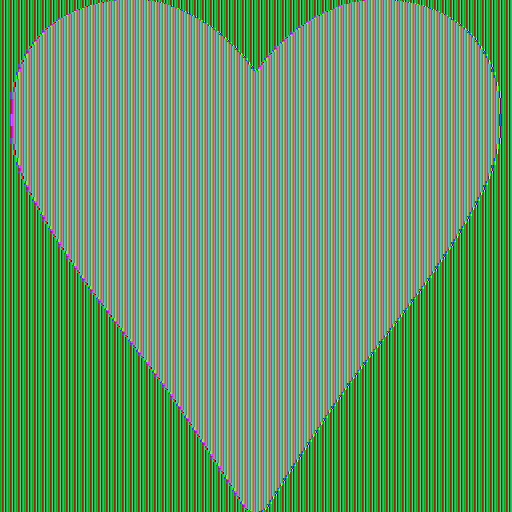
\includegraphics[width=0.5\textwidth]{images/File1.png}
    \caption{File1.ppm}
\end{figure}

\begin{figure}
    \centering
    
\includegraphics[width=0.5\textwidth]{images/File2.png}
    \caption{File2.ppm}
\end{figure}

\begin{figure}
    \centering
    
\includegraphics[width=0.5\textwidth]{images/File3.png}
    \caption{File3.ppm}
\end{figure}

\begin{figure}
    \centering
    
\includegraphics[width=0.5\textwidth]{images/File4.png}
    \caption{File4.ppm}
\end{figure}
\begin{figure}
    \centering
    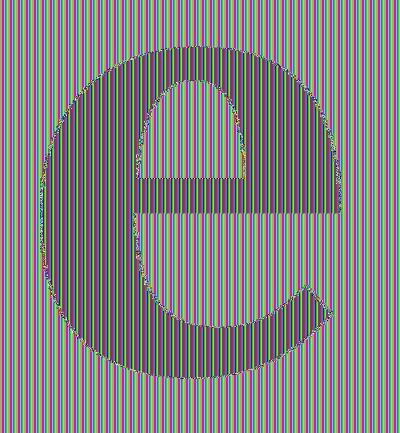
\includegraphics[width=0.5\textwidth]{images/File5.png}
    \caption{File5.ppm}
\end{figure}
\begin{figure}
    \centering
    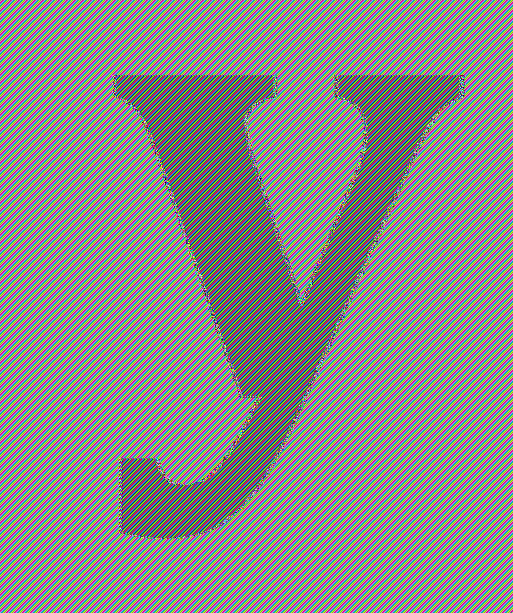
\includegraphics[width=0.5\textwidth]{images/File6.png}
    \caption{File6.ppm}
\end{figure}

\begin{figure}
    \centering
    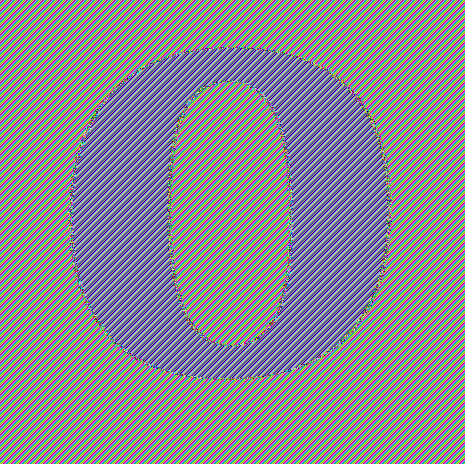
\includegraphics[width=0.5\textwidth]{images/File7.png}
    \caption{File7.ppm}
\end{figure}

\begin{figure}
    \centering
    
\includegraphics[width=0.5\textwidth]{images/File8.png}
    \caption{File8.ppm}
\end{figure}
The plaintext is "$\heartsuit$Loveyou" (I'm not sure about uppercase and lowercase).

\end{document}